\documentclass[a4j]{jarticle}

% tab01.tex
\usepackage[dvipdfmx]{graphicx}

\begin{document}

\begin{table}[htb] %start table (tabular not a table)
    %table* akan memaksa tablenya jadi one column
    % h -> here, t -> top, b -> bottom
    \caption{国別詳細データ} % penamaan table (before the table itself)
    \label{kuni-data}
    \begin{center} % allignment
        \begin{tabular}{|c|c|c|} % c -> center, l or r
            \hline
            \multicolumn{3}{|c|}{各国のデータ}\\ 
            \hline % hline -> horizontal line
            国名&首都&言語\\ 
            \hline
            日本&東京&日本語\\ 
            \hline
            イギリス&ロンドン&英語\\ 
            \hline
            フランス&パリ&フランス語\\
            \hline
            ドイツ&ベルリン&ドイツ語\\
            \hline
        \end{tabular}
    \end{center}
\end{table}

\begin{figure}[htb]
    \begin{center}
        
\includegraphics[scale=0.5]{apple01.png}
        \caption{リンゴのマーク} % dibawah image
        \label{apple_mark}
    \end{center}
\end{figure}

\begin{figure}[htb]
    \begin{center}
        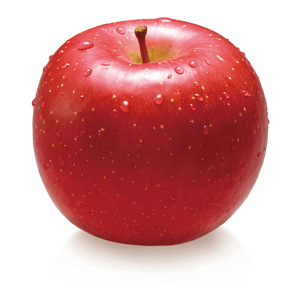
\includegraphics[scale=0.4]{apple02.jpg}
        \vspace{-5mm}
        \caption{リンゴの写真}
        \label{apple_pic}
    \end{center}
\end{figure}

% 国別の詳細を俵~\ref{kuni-data}に掲載する.

表~\ref{kuni-data}は国別の詳細で,図~\ref{apple_mark}はリンゴのマーク,図~\ref{apple_pic}はリンゴの写真である.

    
\end{document}